\documentclass{article}
\usepackage{amsmath}
\usepackage{natbib}
\usepackage{graphicx}
\usepackage{subfig}
\usepackage{bm}
\usepackage{appendix}
\usepackage{authblk}

% Special commands 
\newcommand{\vect}[1]{\boldsymbol{\mathbf{#1}}}
\providecommand{\e}[1]{\ensuremath{\times 10^{#1}}}

\title{Domestic Trade and Inequality}
\author[1]{Farid Farrokhi}
\author[2]{David Jinkins\thanks{We thank Sina Smid for research assistance, and participants in seminars at Copenhagen Business School and Cardiff University for helpful suggestions.}}
\affil[1]{Penn State}
\affil[2]{Copenhagen Business School}
\renewcommand\Authands{ and }

\begin{document}
\maketitle

Inequality has long fascinated economists, and growing income inequality has been heatedly discussed in public forums recently.\footnote{It is not every year that a 700-page collection of charts and academic theory on inequality is a New York Times bestseller.}  In this paper, we add to this discussion by documenting some new facts about the interaction of geography with inequality, and developing a model which can rationalize what we find.  After estimating the model on American data, we will discuss the effect of changes in geography on inequality.  These changes might be a new highway, or population movement due to climate change.

Our first empirical contribution is to document facts about inequality and geography.  We assign to each American city a measure of remoteness meant to capture its distance from all other cities.  We then show that this measure correlates negatively with the skill premium, the ratio of the mean wage of the highly educated to the mean wage of the less educated.  That is, highly educated workers make less relative to less educated workers in remote cities.  On the other hand, conditional on population and other controls, the more remote a city is, the higher its share of highly educated workers, which we call the college share.  As far as we know, our paper is the first to document these facts.

At least since the development of new economic geography, economists have examined the role of trade costs in determining the location of manufacturing centers \textbf{CITE KRUGMAN,allen arkolakis}.  On the other hand, recent models of spatial inequality have treated cities as isolated.  Workers in a city can interact with each other, but there is no interaction between cities.  This literature, then, has no way to discuss the interaction of geography with inequality, since the geographic location of a city relative to other cities is irrelevant.  By including intra-city trade in an model of inequality, we bridge this gap in the literature.

In our model, we have a continuum of locations, workers, and firms.  Workers come in two types, skilled and unskilled, and each worker has an ideosyncratic utility from living in each location.  A worker decides where to live taking wages as given.  A firm also takes local wages as given, and produces a tradable good using skilled and unskilled labor as inputs.  The sole difference between the two types of labor is that skill labor benefits from agglomeration, while unskilled labor does not.\footnote{We allow there to be a Hicks-neutral agglomeration force as well.}

The key in our model is to generate skill premia which differ by location.  In particular, we want less remote cities to have higher skill premia.  Consider a city near other cities.  The access to cheap tradable goods makes this location attractive to live in.  This leads the city to have a relatively high population.  Through agglomeration forces, skilled workers become relatively productive.  Thus, a firm in this city chooses a relatively high share of skilled workers as inputs.  The more skilled workers are attracted to the city, the more difficult it is to attract the marginal skilled worker, since she has a strong preference to live elsewhere.  A high skill premium is necessary in this city to increases the relative supply and decreases the relative demand for skilled workers.

To clarify this mechanism, consider software engineers and gas station attendants.  There are more software engineers per gas station attendant in Silicon Valley than in Minneapolis.  Agglomeration effects make software engineers much more productive in Silicon Valley, but gas station attendents are almost the same productivity everywhere.  Thus, Silicon Valley demands relatively more software engineers.  In order to both increase Silicon Valley relative supply of software engineers and reduce relative demand, we need to make the software engineer wages in Silicon Valley relatively high compared with gas station attendants.

The literature on the skill premium has found a number of patterns.  To the extent that we are able to measure the relevant quantities, all of these facts are consistent with our data.  The literature has shown convincingly that the skill premium is higher in cities with larger populations \citep{davis2012spatial}.  The relationship between the skill premium and city size has become stronger over time \citep{baum2013inequality, lindley2014spatial}.  In addition, larger cities have been shown to have a higher share of college-educated worker, another pattern which has strengthened over time \citep{moretti2008real, lindley2014spatial}.  Areas of denser economic activity have higher skill premiums \citep{combes2012sorting}.

These stylized facts have generated a number of theories to help understand them \citep{davis2012spatial,davis2014comparative,baum2012understanding,combes2012sorting}.  These theories abstract from costly trade, treating trade between cities as either non-existant or frictionless.\footnote{\citet{davis2012spatial} does contain an extension where trade costs are treated in the limit as they go to zero.}  The style of our modeling exercise below has more in common with recent forays of trade economists into economic geography \citep{allen2014trade,desmet2014geography}.  These theories model costly trade, and focus on the spatial location of economic activity. They have, however, only one type of labor, so they cannot analyze the interaction between geography and inequality.  In an international trade context, \citet{fujita2006globalization} study inequality with costly trade, but their model has immobile unskilled workers.

\textbf{ADD THE PhD guy, and maybe a moretti paper or two more}

\section{Documenting inequality and geography}

In this section, we describe our data sources, give our definitions of measures of geography and inequality, and present the empirical findings which motivate our modeling exercise.  
\subsection{Data sources}

Our empirical section is based on data from the 2000 American census public use micro-data (PUMS).  In order to be consistent with the literature, we clean the data using replication code from Baum-Snow ReStat, which is available on Nathanial Baum-Snow's website.  In this cut of the data, we eliminate all workers except for white males older than 24 and younger than 55 to abstract from any considerations of sex or race discrimination.  As it stands we are left with around 1.5 million workers distributed across the United States.

We want to compare inequality in different locations.  For our purposes, a location will be a 2000 US Census Metropolitan Statistical Area (MSA).  There are more than 300 MSAs, which are economically-integrated regions.  The borders of these regions are based on county borders.  Not all American counties are part of an MSA.  In order to think about the geography of MSA's, we need to know the precise location of each MSA in space.  We download a population weighted centroid for each MSA (and PMSA) from the Missouri census data center (http://mcdc2.missouri.edu/websas/geocorr2k.html).

\subsection{Important concepts}

Our main measure of geography is remoteness, a concept we borrow from the international trade literature.\footnote{It is a famous empirical regularity that the trade of two countries is proportional to the product of their national products divided by the physical distance between them.  This relationship is known as the naive gravity equation.  The adjective naive makes an appearance because such a gravity equation implies that trade between two countries is unaffected by what takes place in a third country.  For example, the trade between the United States and Mexico is unaffected by the rapid increase in trade between China and the United States.  Remoteness in an international trade context is the national-product-weighted sum of the distance between a country and all other countries.  Multiplying the gravity equation by a remoteness term allows third countries to influence bilateral trade relationships.}  The particular functional form we use is based on a suggestion in \citet{head2003gravity}.  Let us label each MSA with a number $i=1\dots N$.  The population of MSA $i$ is $P_i$, and the geodesic distance, i.e. the distance as the crow flies, between MSA $i$ and MSA $j$ is $d_{i,j}$.  The remoteness of MSA $i$ $R_i$ is given by:

\begin{equation}
    R_i = \frac{1}{\sum_{j\neq i} \frac{P_j}{d_{i,j}}} \nonumber
    \label{eq:rem}
\end{equation}

In words, an MSA which is close to other MSA's with high populations will have low remoteness.  We want this measure to reflect the ease with which a location can trade with other locations.  This measure does not, of course, take into account geographic features such as rivers, mountains, roads, and airports, but physical distance is still an important part of transportation cost.  

We have two measures of inequality, the skill premium and the college share.  Both are measured in a way standard in the labor literature, and are calculated in each MSA.  A worker is highly educated if he has either a college degree or an academic associate degree.  The skill premium is the mean wage of highly-educated workers in an MSA divided by the mean wage of other workers.  The college share is the fraction of highly-educated workers in an MSA.  When calculating all means, we use census population weights.

In addition to our inequality variables, we define the age ratio to be the mean age of the highly educated divided by the mean age of the less educated.  Since we know from the labor literature that wages rise dramatically with age, it will be important for us to control for differences in the age profile of the two education groups in our analysis.  Ideally, we would run our analysis using only workers of approximately the same age, but such a cut reduces the size of our data dramatically and causes measures of inequality to be unreliable in smaller MSA's.  For example, including only workers within a 15-year age window reduces our data by more than half.  While it is somewhat dependent on which specific ages we choose, we get similar results in terms of both magnitudes and statistical significance if we restrict our sample to a 15-year age window rather than including age ratio as a regressor.

Table \ref{tab:sum_stats} contains some descriptive statistics.  Figure \ref{fig:geo} shows how our measures vary across the United States. In each of these figures, blue signifies a higher quantity, and red a lower quantity.  Remoteness has an obvious geographic pattern, as does the skill premium.  Remoteness is lowest in regions radiating out from New York and Chicago.  The skill premium is higher on the East Coast and in the South than it is in the Midwest and the Pacific Northwest.  It is more difficult to see an obvious geographic pattern in college share and population, except that both are higher in New England, the Pacific Northwest, and the coast of California.

\begin{table}
    \centering
    \begin{tabular}{lll}
        \hline \hline
        Statistic & Mean & Standard Dev \\ 
        \hline
        Remoteness    & 3.6\e{-6} & 1.8\e{-6} \\
        Population    & 7.3\e{5}  & 1.2\e{6}  \\
        Skill premium & 1.7       & 0.18      \\
        College share & 0.46      & 0.22      \\
        Age ratio     & 1.03      & 0.03      \\
        \hline
        Census observations & 1.1\e{6} & \\
        MSA observations    & 309      & \\
        \hline \hline
    \end{tabular}
    \caption{Data summary statistics}
    \label{tab:sum_stats}
\end{table}

\begin{figure}[!ht]
  \centering
  \subfloat[Remoteness]{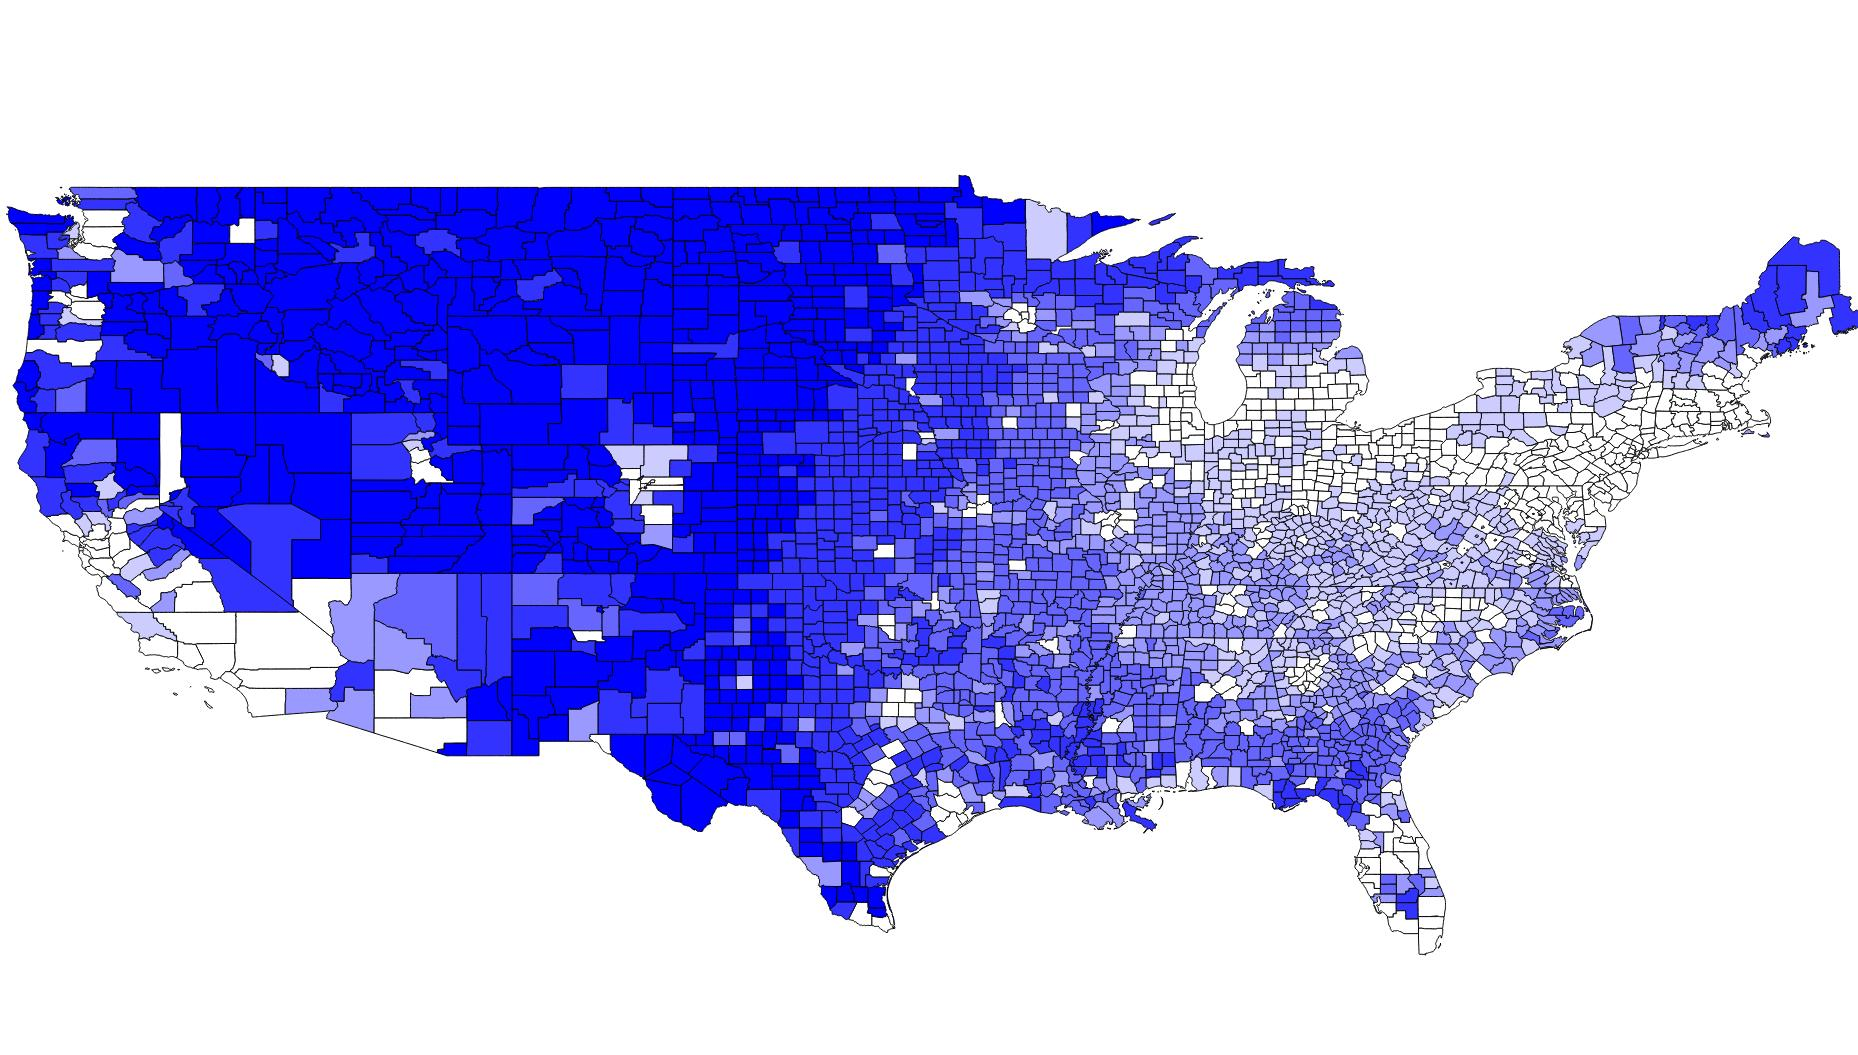
\includegraphics[width=.47\textwidth]{pics/rem.jpeg}}\quad
  \subfloat[Population]{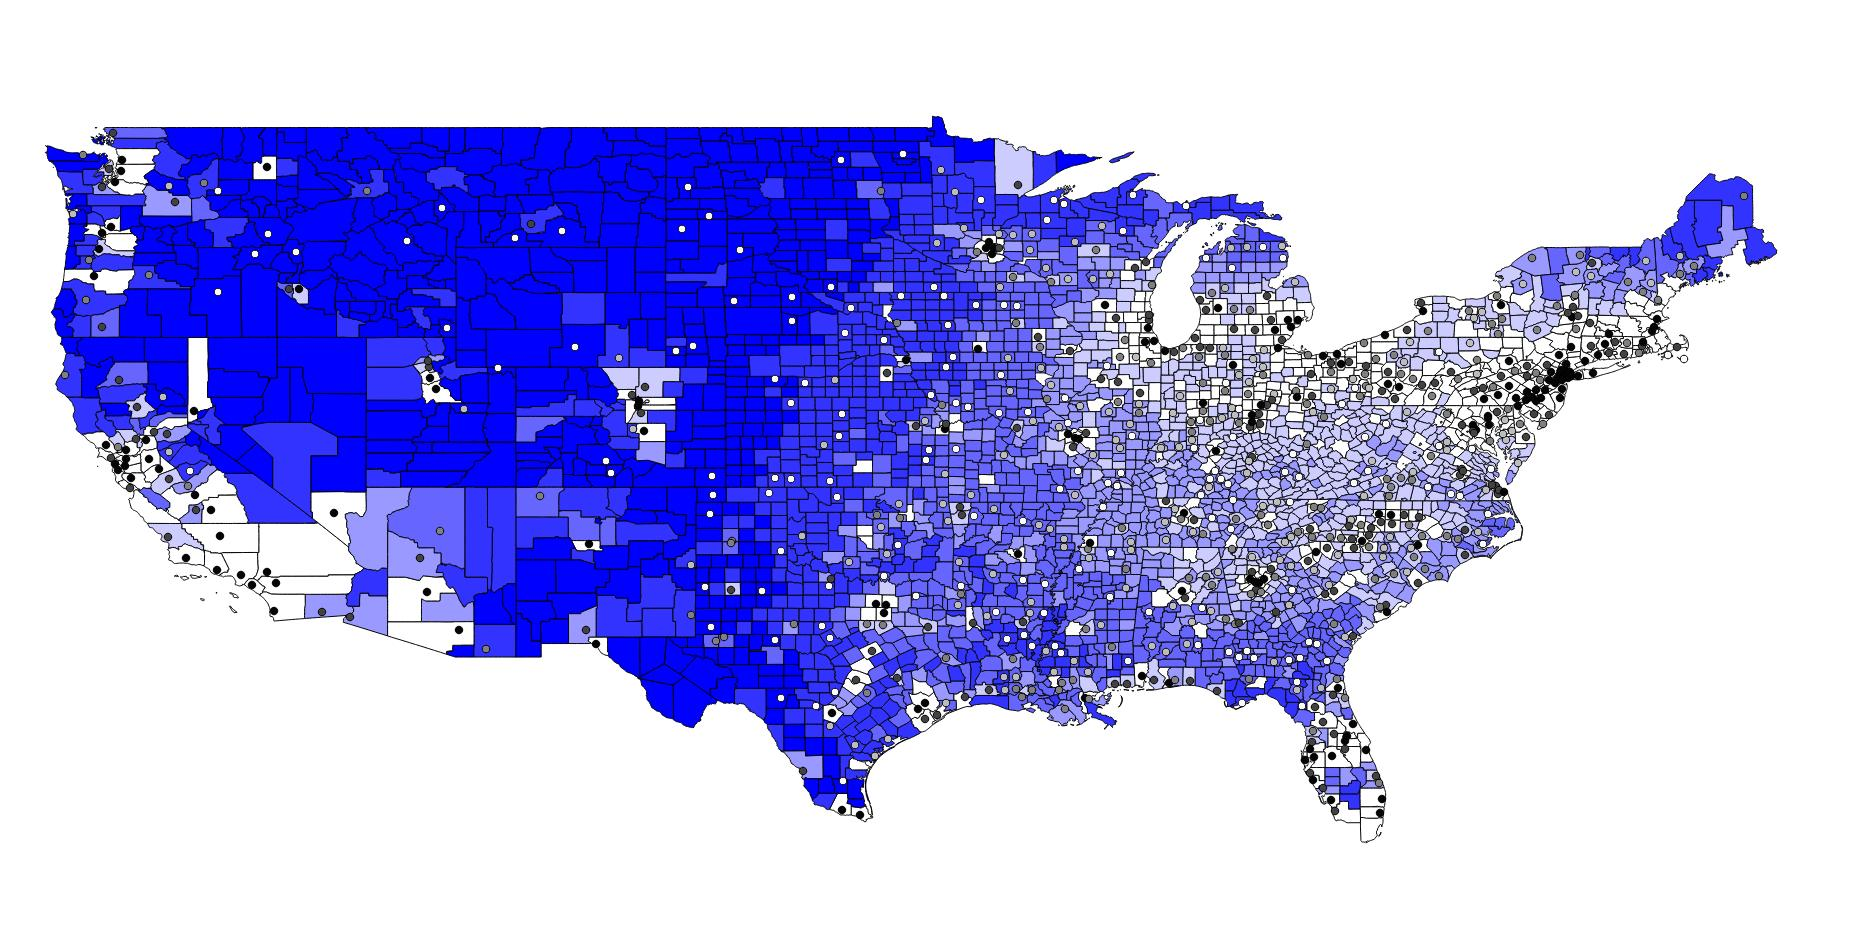
\includegraphics[width=.47\textwidth]{pics/pop.jpeg}}\\
  \subfloat[Skill Premium]{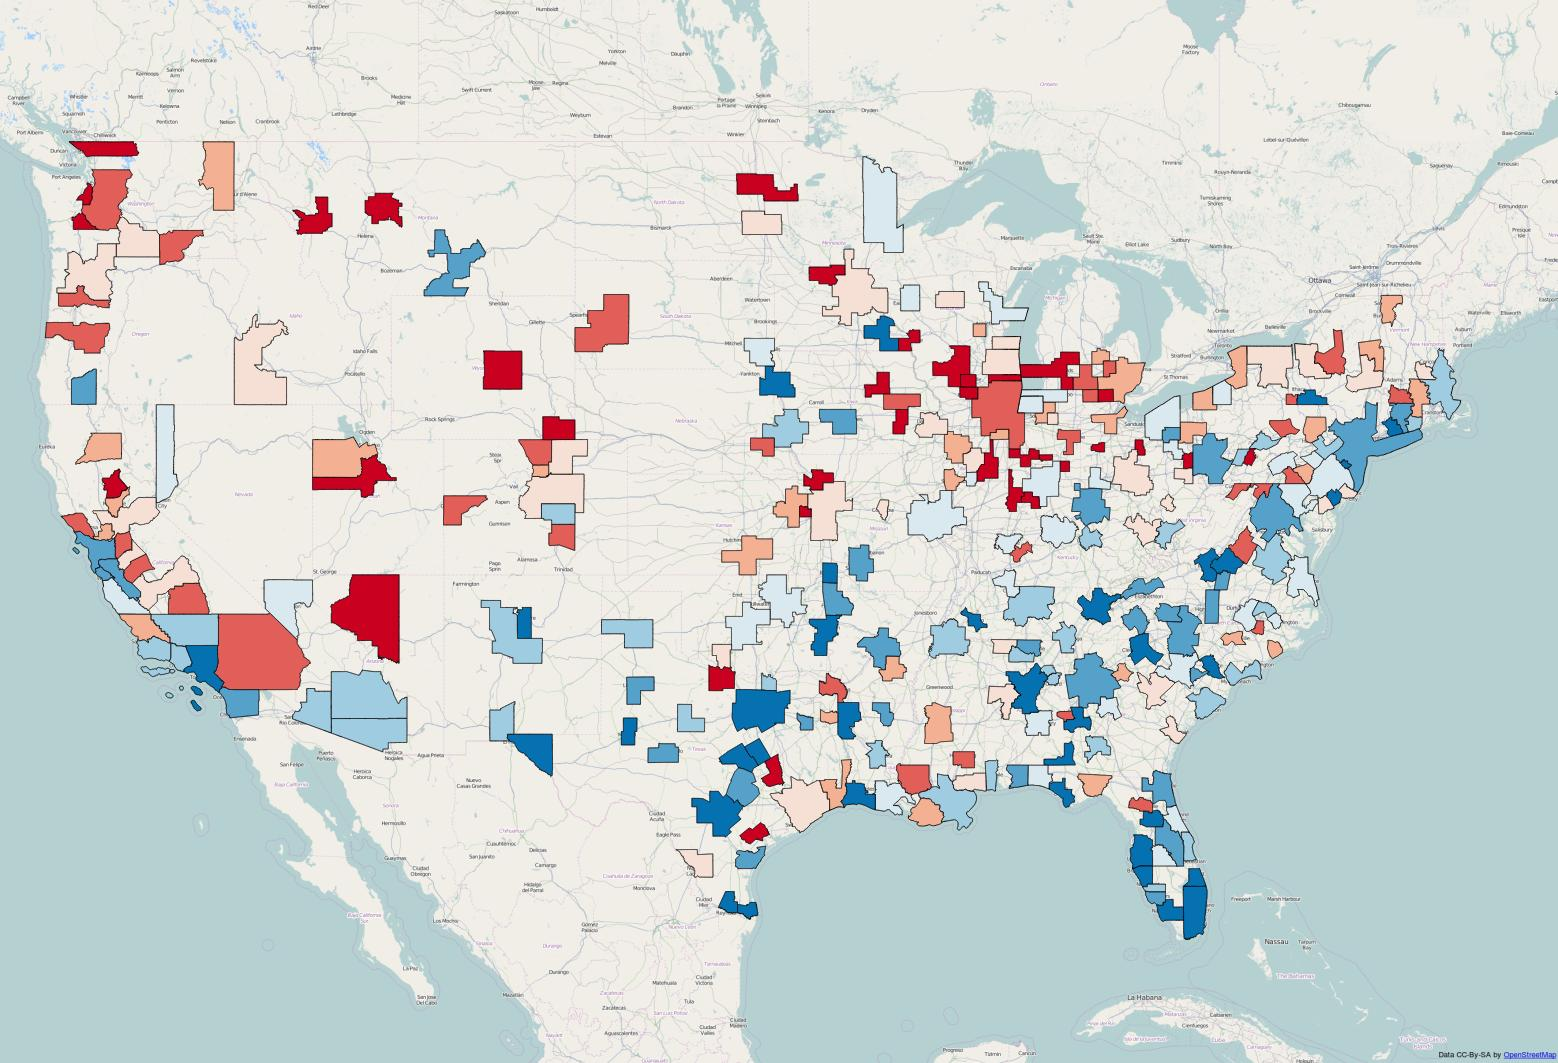
\includegraphics[width=.47\textwidth]{pics/skill_prem.jpeg}}\quad
  \subfloat[College Share]{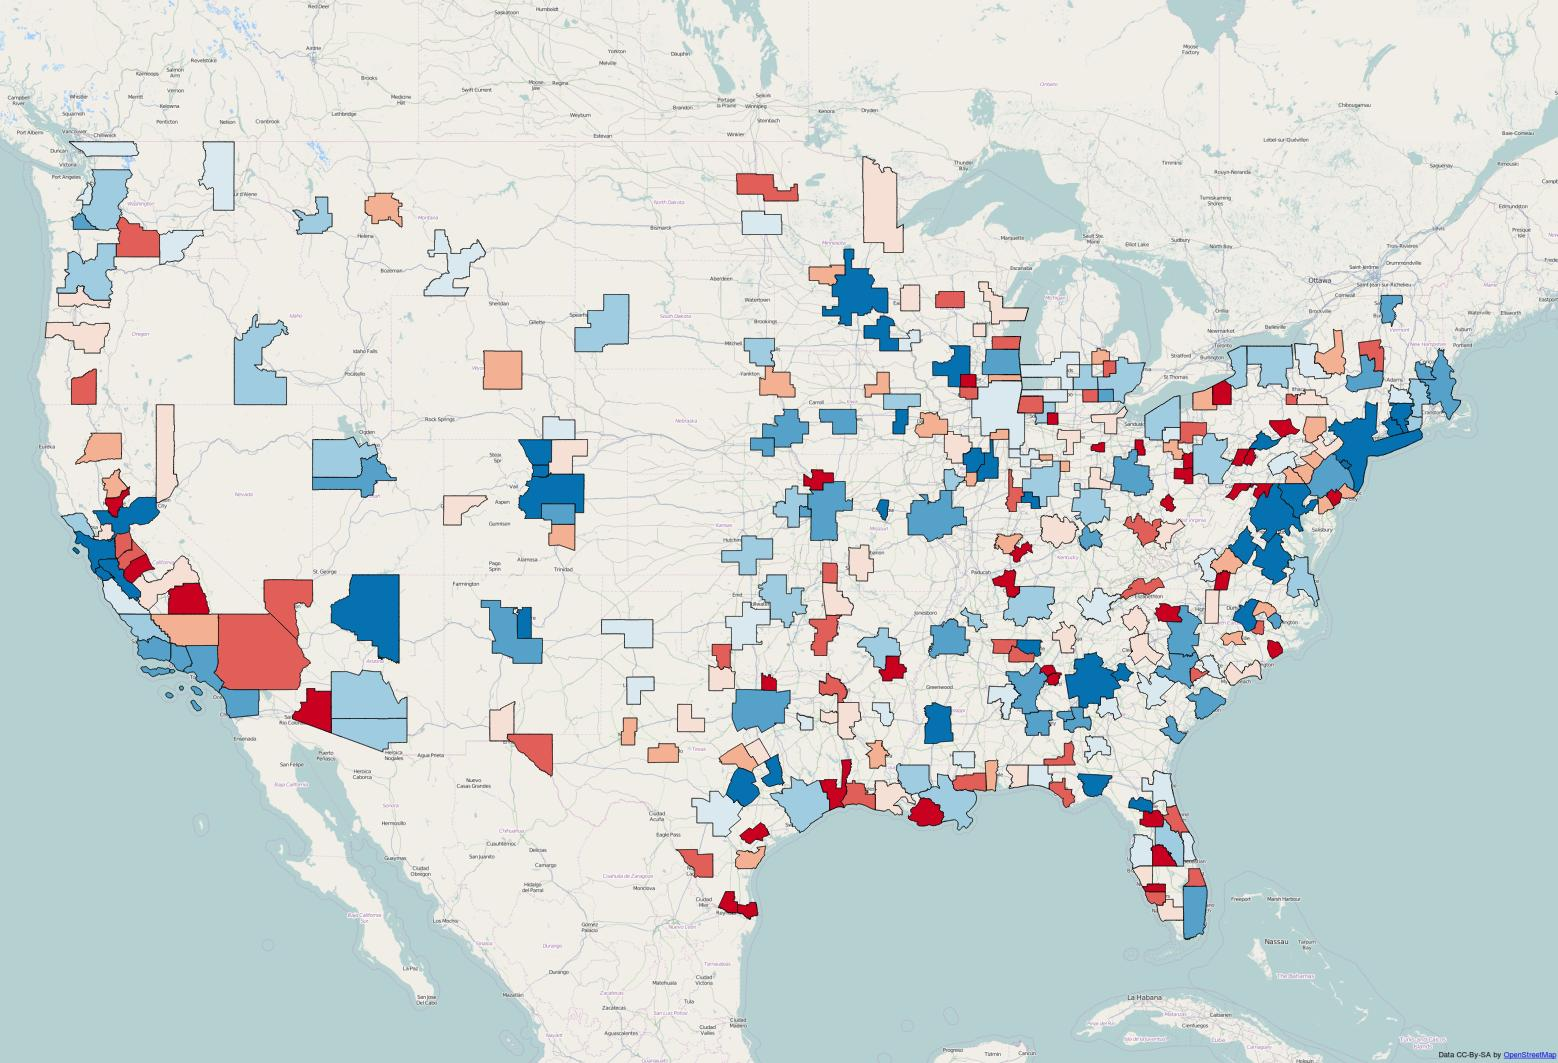
\includegraphics[width=.47\textwidth]{pics/college_ratio.jpeg}}
  \caption{MSA's by data feature}
  \label{fig:geo}
\end{figure}

\subsection{Empirical results}

% This table was done using estout package in stata, which is why the code looks so ugly!
\begin{table}
    \centering
    {
    \def\sym#1{\ifmmode^{#1}\else\(^{#1}\)\fi}
    \begin{tabular}{l*{3}{c}}
    \hline\hline
                        &\multicolumn{1}{c}{(1)}&\multicolumn{1}{c}{(2)}&\multicolumn{1}{c}{(3)}\\
                        &\multicolumn{1}{c}{Ln Skill Prm}&\multicolumn{1}{c}{Ln Skill Prm}&\multicolumn{1}{c}{Ln Skill Prm}\\
    \hline
    Ln Remote           &     -0.0133         &     -0.0452\sym{**} &     -0.0493\sym{***}\\
                        &    (0.0161)         &    (0.0180)         &    (0.0165)         \\
    [1em]
    Ln Age Rat          &                     &       0.997\sym{***}&       1.388\sym{***}\\
                        &                     &     (0.272)         &     (0.255)         \\
    [1em]
    Ln Pop              &                     &                     &      0.0411\sym{***}\\
                        &                     &                     &   (0.00535)         \\
    [1em]
    Constant            &       0.370\sym{*}  &     -0.0617         &      -0.653\sym{***}\\
                        &     (0.203)         &     (0.232)         &     (0.226)         \\
    \hline
    Observations        &         309         &         309         &         309         \\
    Adjusted \(R^{2}\)  &      -0.001         &       0.038         &       0.191         \\
    \hline\hline
    \multicolumn{4}{l}{\footnotesize Standard errors in parentheses}\\
    \multicolumn{4}{l}{\footnotesize \sym{*} \(p<0.10\), \sym{**} \(p<0.05\), \sym{***} \(p<0.01\)}\\
    \end{tabular}
    }
    \caption{Regressions of log skill premium on log geography variables}
    \label{tab:skill_reg}
\end{table}


% This table was done using estout package in stata, which is why the code looks so ugly!
\begin{table}
    \centering
    {
    \def\sym#1{\ifmmode^{#1}\else\(^{#1}\)\fi}
    \begin{tabular}{l*{3}{c}}
    \hline\hline
                        &\multicolumn{1}{c}{(1)}&\multicolumn{1}{c}{(2)}&\multicolumn{1}{c}{(3)}\\
                        &\multicolumn{1}{c}{Ln College Shr}&\multicolumn{1}{c}{Ln College Shr}&\multicolumn{1}{c}{Ln College Shr}\\
    \hline
    Ln Remote           &     -0.0209         &       0.199\sym{***}&       0.182\sym{***}\\
                        &    (0.0650)         &    (0.0696)         &    (0.0632)         \\
    [1em]
    Ln Age Rat          &                     &      -6.880\sym{***}&      -5.289\sym{***}\\
                        &                     &     (1.052)         &     (0.974)         \\
    [1em]
    Ln Pop              &                     &                     &       0.167\sym{***}\\
                        &                     &                     &    (0.0205)         \\
    [1em]
    Constant            &      -1.131         &       1.846\sym{**} &      -0.557         \\
                        &     (0.821)         &     (0.894)         &     (0.863)         \\
    \hline
    Observations        &         309         &         309         &         309         \\
    Adjusted \(R^{2}\)  &      -0.003         &       0.117         &       0.273         \\
    \hline\hline
    \multicolumn{4}{l}{\footnotesize Standard errors in parentheses}\\
    \multicolumn{4}{l}{\footnotesize \sym{*} \(p<0.10\), \sym{**} \(p<0.05\), \sym{***} \(p<0.01\)}\\
    \end{tabular}
    }
    \caption{Regressions of log college share on log geography variables}
    \label{tab:col_reg}
\end{table}

In this section we document the covariance of our measure of geography, remoteness, with our measures of inequality, the skill premium and college share.  Regressions of the skill premium on remoteness and other variables are found in Table \ref{tab:skill_reg}.  Remoteness covaries negatively with the skill premium, although the coefficient is not significant untless the age ratio is included in the regression.  We find that the population of an MSA varies positively with the skill premium, a result that has been emphasized in other studies.  The covariance of remoteness and the skill premium is nearly the same size as its covariance with population, but in the opposite direction.

In Table \ref{tab:col_reg} we report coefficient estimates from regressions of college ratio on the same regressors.  We find that remoteness covaries positively with the college premium, and as before the effect is only significant after controling for the age ratio.  This effect is surprising, as one might expect highly-educated workers to be disproportionately drawn to large cities in areas with low remoteness.  On the other hand, it makes sense that in remote areas where the skill premium is lower, we should find a larger relative supply of highly-educated workers.  As before, the magnitude of the population effect and the remoteness effect are similar.

We have strong intuition for why the age ratio is positively correlated with the skill premium.  Older people earn more, so if highly-educated workers are older than less-educated workers, the skill premium will be higher.  We do not have such strong intuition for the strong negative correlation between the college share and the age ratio.  In words, MSA's with a high fraction of highly-educated workers, have relatively young highly-educated workers.

An alternative method of controling for the age of workers is to limit our analysis to workers in a smaller age range.  Doing this significantly reduces the data available for us to calculate our regressors accurately.  As a robustness check, we present results in the appendix for only workers 35 to 50 years old.  The results are nearly the same as those found in our main analysis.

\section{Theory}

In the last section, we presented evidence that geography plays a role in shaping the skill premium and college shares.  In this section we develop an empirical model to help us understand the patterns we found, in particular that the skill premium decreases with the remoteness of a location, while the college share increases.  Next we discuss how such a model might be estimated.

\subsection{Labor Supply}

We have a static model with a continuum of price-taking firms in each location, and two types of worker: skilled indexed by $H$, and unskilled indexed by $L$.  The utility of a worker in location $i$ is:
\begin{eqnarray}\label{eq:utility}
	Q(i) u(i) \epsilon(i)
\end{eqnarray} 
where $Q(i)$ is utility from tradeables, $u(i)$ is the utility from exogenous amenities, and $\epsilon(i)$ is a worker's exogenous preference for location $i$.  Tradeable goods are differentiated by the origin of production, and $q(j,i)$ is consumer's consumption in $i$ from goods originated in location $j$. The aggregator $Q(i)$ in the utility function with $\sigma>0$ the elasticity of substitution is:
\[
	Q(i) = \left[\int_J q(j,i)^{\frac{ \sigma - 1}{\sigma}}~ dj\right]^{\frac{\sigma}{\sigma-1}},
\]
We suppose that worker location prefrences $\epsilon(i)$ are independent across workers and locations, and have a Type II Extreme Value distribution,
\[
\Pr(\epsilon^h(i) \leq \epsilon) = \exp(-\epsilon^{-\theta})
\]
Workers are heterogeneous in terms of skill $s \in \{H,L\}$. A worker's wage in location $i$ is denoted by $w_s(i)$, and her budget constraint is 
\begin{eqnarray}\label{eq:budget}
	w_s(i) = \int_J p(j,i)q(j,i)~dj 
\end{eqnarray}
where $p(j,i)$ is price of good $j$ in destination $i$, and $J$ is the given set of locations.

An worker has two types of decision to make.  She decides where to live, and how much of each good to consume.  Given a choice of location, the second problem is standard.  A worker of type $s$ in location $i$ spends $x_s(j,i)$ on goods produced in $j$,
\begin{eqnarray}\label{eq:x_s}
	x_s(j,i) & \equiv & p(j,i) q_s(j,i) = \Big[ \frac{p(j,i)}{P(i)} \Big]^{1-\sigma} w_s
\end{eqnarray}
where $P(i)$ is the CES price index,
\begin{eqnarray}\label{eq:price_index}
	P(i) = \left[\int_J p(j,i)^{1-\sigma}~ dj\right]^{\frac{1}{1-\sigma}}
\end{eqnarray}

The second decision a worker makes is where to live.  In order to characterize this decision, we need to introduce congestion forces.  We model them as in \textbf{allen arkolakis}:
\begin{eqnarray}\label{eq:congestion}
u(i) = \bar{u}(i)  n(i)^{\gamma}
\end{eqnarray}
Here, $n(i)$ is total population in location $i$ and $\gamma<0$ is the degree of congestion effect. This specification is isomorphic to a setting where preferences are Cobb-Douglas between tradeables and housing in which housing supply is inelastic.
A worker with skill level $s$ faces the following discrete choice problem over locations:
\begin{eqnarray} 
\max_{i \in J}~ \frac{w_s(i)}{P(i)}u(i) \epsilon(i)  \nonumber
\end{eqnarray}
Using the properties of the Type-II extreme value distribution, within skill $s$ the ratio of labor supply equals
\begin{eqnarray}
	\frac{n_s(i)}{n_s(j)} = 
	\Big[
	\frac{w_s(i)u(i)/P(i)}
	{w_s(j)u(j) /P(j)}
	\Big]^{\theta} \nonumber  
\end{eqnarray} 
where $n_s(i)$ is population of workers with skill $s$ in location $i$.
The elasticity of relative labor supply to relative wages is:
\[
\frac{ \partial \Big(n_s(i)/n_s(j)\Big) \Big/
\Big(n_s(i)/n_s(j)\Big)}
{\partial \Big(w_s(i)/w_s(j)\Big) \Big/
\Big(w_s(i)/w_s(j)\Big) } = \theta
\]
The variance of $\epsilon^h(i)$ is a decreasing function of $\theta$: the larger $\theta$, the smaller the variance. A larger $\theta$ implies that individual unobserved preferences for location are less important, and so workers are more willing to move in response to differences in wages, prices, or amenities ---supply curve is relatively flat.
When $\theta$ is smaller, the variance is large, so supply curve is relatively steep: A larger change in wages is needed to attract one more percentage of workers. 

Not all but marginal workers are indifferent between locations. For all $i \in J$, for each skill level, we define $W_s$ as the utility of the marginal worker,
\begin{eqnarray}\label{eq:indiff}
	 W_s \equiv \frac{w_s(i)} {P(i)} u(i) n_s(i)^{-1/\theta}
\end{eqnarray}

\subsection{Labor Demand}
Each location has a representative firm with a CES production function using high- and low skill workers,
\begin{eqnarray}
	 A(i)\Big[ \beta_H(i) n_H(i)^{\frac{\varepsilon-1}{\varepsilon}} + \beta_L(i) n_L(i)^{\frac{\varepsilon-1}{\varepsilon}} \Big]^{\frac{\varepsilon}{\varepsilon-1}} \nonumber
\end{eqnarray}
where $A(i)$ is total factor productivity in location $i$. $\varepsilon>0$ is the elasticity of substitution between high and low skill workers. $\beta_H(i)>0$ and $\beta_L(i)>0$ are factor intensities. In the model, differences in factor productivity is the \textit{only} determinant of skill.
By cost minimization, the unit cost of production equals
\begin{eqnarray}\label{eq:unit_cost}
	 \frac{c(i)}{A(i)} ,~where~~c(i)=\Big[ \beta_H(i)^{\varepsilon} w_H(i)^{1-\varepsilon} + \beta_L(i)^{\varepsilon} w_L(i)^{1-\varepsilon}\Big]^{\frac{1}{1-\varepsilon}}
\end{eqnarray}
Share of spending of producers on high skill workers, denoted by $b(i)$, is given by
\begin{eqnarray}\label{eq:input_share}
	b(i) = \frac{\beta_H(i)^{\varepsilon} w_H(i)^{1-\varepsilon}}{\beta_H(i)^{\varepsilon} w_H(i)^{1-\varepsilon} + \beta_L(i)^{\varepsilon} w_L(i)^{1-\varepsilon}}
\end{eqnarray}
Following the literature, we distinguish two sorts of agglomeration forces. First 
\begin{eqnarray}\label{eq:agglom_general}
A(i) = \bar{A}(i) n(i)^{\alpha}
\end{eqnarray}
with $\alpha>0$. This agglomeration force changes productivity of both low and high skill workers. A Krugman type monopolistic competition generates similar force through endogenous measure of firms. In addition, there is overwhelming evidence that agglomeration forces are stronger for high skill workers; suggesting that high skill individuals are more productive through exchanging ideas with each other. Motivated by these findings, we let a high skill individual be more productive through concentration of high skill workers,
\begin{eqnarray}\label{eq:agglom_specific}
	\beta_H(i) & = & \bar{\beta}_H(i) n_H(i)^{\varphi} \nonumber \\
	\beta_L(i) & = & \bar{\beta}_L(i)
\end{eqnarray}
[skilled-biased technological change, motivated by the fact that population share of high-skilled is higher in locations where skill premium is also higher]


Finally, markets are perfectly competitive. Let $d(j,i)$ be the trade costs of shipping a good from $j$ to $i$. Price of a good produced in location $j$ and consumed in location $i$, $p(j,i)$, equals $c(j)d(j,i)/A(j)$. 

\subsection{Equilibrium}

Definition. A \textit{spatial equilibrium} is a set of $w_H(i)$, $w_L(i)$, $n_H(i)$, and $n_L(i)$ such that
\begin{itemize}
\item Goods market clear
\begin{eqnarray}\label{eq:goods_mkt_clear}
	w_H(i) n_H(i) =  b(i) \int_J \sum_{s \in \{H,L\}} n_s(i)x_s(j,i) ~dj 
\end{eqnarray}
where $x_s(j,i)$ is given by (\ref{eq:x_s}), and $b(i)$ is given by (\ref{eq:input_share}).
\item Marginal workers are indifferent across locations according to (\ref{eq:indiff}).
\item Feasible allocation of labor, $\int_J n_H(j) ~dj = N_H$ and $\int_J n_L(j) ~dj = N_L$.
\end{itemize}

\vspace{5mm}
\textit{Equilibrium Analysis.}~~ On the demand side of labor markets, 
\begin{eqnarray}
	b(i) \equiv \frac{1}{1 + \frac{n_L(i)}{n_H(i)} \frac{w_L(i)}{w_H(i)}} = \frac{1}{1 + \Big(\frac{\beta_L(i)}{\beta_H(i)}\Big)^{\varepsilon} \Big(\frac{w_L(i)}{w_H(i)}\Big)^{1-\varepsilon}} \nonumber
\end{eqnarray}
where the LHS is an equivalent definition for high skill input share, and the RHS is equivalent to (\ref{eq:input_share}). Therefore,
\begin{eqnarray}\label{eq:labor_demand_general}
	\Big[\frac{\beta_L(i)}{\beta_H(i)}\Big]^{\varepsilon} \Big[\frac{w_L(i)}{w_H(i)}\Big]^{-\varepsilon}= \frac{n_L(i)}{n_H(i)} 
\end{eqnarray}
Under our specification, equation (\ref{eq:labor_demand_general}) yields
\begin{eqnarray}\label{eq:labor_demand}
	\omega(i) \equiv \frac{w_H(i)}{w_L(i)} = \frac{\bar{\beta}_H(i)}{\bar{\beta}_L(i)}\Big[ \frac{n_H(i)}{n_L(i)} \Big]^{-1/\varepsilon}n_H(i)^{\varphi/\varepsilon}
\end{eqnarray}
where $\omega(i)$ is skill premium in location $i$.

According to welfare equalization for marginal workers, equation (\ref{eq:indiff}), the supply side of labor markets imply
\begin{eqnarray}\label{eq:labor_supply}
	\omega(i) = \frac{W_H}{W_L} \Big[ \frac{n_H(i)}{n_L(i)} \Big]^{\theta}
\end{eqnarray}
Labor markets clear when skill premia, $[\omega(i)]_{i \in J}$, satisfy the pairs of demand by (\ref{eq:labor_demand}) and supply by (\ref{eq:labor_supply}). By equations \ref{eq:labor_demand}--\ref{eq:labor_supply},
\begin{eqnarray}\label{eq:labor_demand_supply}
n_L(i) = \Big( \frac{W_L}{W_H} \frac{\bar{\beta}_H(i)}{\bar{\beta}_L(i)} \Big)^{-\varepsilon/(1+\theta \varepsilon)} \Big( n_H(i) \Big)^{1-\varphi/(1+\theta \varepsilon)}
\end{eqnarray}
Skill share, $n_H/n_L$, is determined solely by exogenous parameters if $\varphi=0$. Skill premium, $w_H/w_L$, equalizes across locations if $\theta=\infty$. In case $\varphi=0$, high skill workers have no advantage from agglomeration effects. Spatial variations in skill share is endogenously derived by skill-specific agglomeration, but this alone does not translate to variations in skill premia. We also need $\theta$ to be finite, or equivalently the variance of unobserved preferences to be positive. When the variance is larger, workers are less willing to migrate in response to changes in wages.
Suppose because of agglomeration effects for high skill workers, there is more demand to attract high skill workers. When unobserved preferences do matter, high skill workers do not fully capitalize this opportunity as some of them are so attached to certain cities. In this respect, our model departs from Rosen-Roback-AA by highlighting the role of labor supply elasticity ---not \textit{all} but only the \textit{marginal worker} is indifferent between locations; and the interaction of labor supply elasticity with the density of high skill workers.

Define $\rho_H(i) = n_H(i)/N_H$ as the density of high skill labor. Equation (\ref{eq:labor_demand_supply}) and $ N_L = \int_J n_L(i)~di $ pin down $W_H/W_L$ only as a function of $\rho_H(i)$,
%\begin{eqnarray}
%\frac{W_H}{W_L} =
%\Big(N_L\Big)^{(1+\theta \varepsilon)/\varepsilon}\Bigg[ \int_J \Big(  \frac{\bar{\beta}_H(i)}{\bar{\beta}_L(i)} \Big)^{-\varepsilon/(1+\theta \varepsilon)} \Big( n_H(i) \Big)^{1-\varphi/(1+\theta \varepsilon)}~di \Bigg]^{-(1+\theta \varepsilon)/\varepsilon}
%\end{eqnarray}
\begin{eqnarray}\label{eq:WHtoL}
\frac{W_H}{W_L} =
\underbrace{\Big(N_H/N_L\Big)^{-(\theta+ \varepsilon)/\theta\varepsilon}}_{\mbox{scarcity}} \times \underbrace{N_H^{\varphi/\varepsilon}}_{\mbox{agglom.}} 
\times
\underbrace{\Bigg[ \int_J \Big( \frac{\bar{\beta}_H(i)}{\bar{\beta}_L(i)} \Big)^{-\theta\varepsilon/(\theta+\varepsilon)} \Big( \rho_H(i) \Big)^{(\theta(1-\varphi)+\varepsilon)/(\theta+\varepsilon)}~di \Bigg]^{-(\theta+ \varepsilon)/\theta\varepsilon}}_{\mbox{allocation}} 
\end{eqnarray}
Equation (\ref{eq:WHtoL}) decomposes the three forces behind real well-being inequality of marginal workers: 1) Aggregate scarcity of high skill labor, 2) Aggregate agglomeration advantage of high skill workers, 3) A weighted average of relative productivities in which weights are the density of high skill labor. While the  first two behave at the aggregate, the third relates to the distribution of population. In addition, note that agglomeration is less effective when the elasticity of substitution between high and low skill labor, $\varepsilon$, is higher.

\textit{Integral Equations.}~~Total income in $i$ equals
$\frac{1}{b(i)} w_H(i)n_H(i)$. Using goods market clearing condition by equations (\ref{eq:goods_mkt_clear}), 
\begin{eqnarray}
	w_H(i) n_H(i) b(i)^{-1} = 
	\int_J \Big[ \frac{c(i) d(i,j)}{A(i) P(j)} \Big]^{1-\sigma} w_H(j) n_H(j) b(j)^{-1} ~dj \nonumber
\end{eqnarray}

Equations (\ref{eq:unit_cost}) and (\ref{eq:input_share}) imply that 
\begin{eqnarray}\label{eq:ctilde}
	c(i) & = & \tilde{c}(i) w_H(i) \nonumber \\
	where~~~ \tilde{c}(i) & = & 
	\Big[\bar{\beta}_H(i) n_H(i)^{\varphi}\Big] ^{\frac{\varepsilon}{1-\varepsilon}} \Big[b(i)\Big]^{\frac{-1}{1-\varepsilon}}
\end{eqnarray}
We replace for $c(i)$ from (\ref{eq:ctilde}) and price index from welfare equalization for marginal workers (\ref{eq:indiff}) into the integral equation. After some algebra,
\begin{eqnarray}\label{eq:system1}
	& & A(i)^{1-\sigma} \tilde{c}(i)^{\sigma-1} n_H(i)  w_H(i)^{\sigma}  b(i)^{-1}  \nonumber \\
	& & =  
	W_H^{1-\sigma}
	\int_J d(i,j)^{1-\sigma} u(j)^{\sigma-1} n_H(j)^{(\theta+1-\sigma)/\theta} w_H(j)^{\sigma} b(j)^{-1}  ~dj
\end{eqnarray}
By replacing price index from welfare equalization (\ref{eq:indiff}) into (\ref{eq:price_index}) 
\begin{eqnarray}
	\Big[ \frac{w_H(i) u(i) n_H(i)^{-1/\theta}}{W_H } \Big]^{1-\sigma} = \int_J c(j)^{1-\sigma}d(j,i)^{1-\sigma}A(j)^{\sigma-1}~ dj \nonumber
\end{eqnarray}
which results
\begin{eqnarray}\label{eq:system2}
 	& &  u(i)^{1-\sigma} n_H(i)^{(\sigma-1)/\theta} w_H(i)^{1-\sigma}  = \nonumber \\ 
 	& & 
 	W_H^{1-\sigma}
 	\int_J  d(j,i)^{1-\sigma} A(j)^{\sigma-1}  \tilde{c}(j)^{1-\sigma} w_H(j)^{1-\sigma}
 	~ dj
\end{eqnarray}
Equations \ref{eq:system1}--\ref{eq:system2} give us two systems of integral equations. Note that in case $\varphi=0$ and $\theta=\infty$, the integral equations collapse to Allen and Arkolakis (2014). 

By the following relation, we can reduce the two systems into one: 
\begin{eqnarray}\label{eq:systems_relation}
	\frac{w_H(i)^{\sigma}n_H(i)A(i)^{1-\sigma}\tilde{c}(i)^{\sigma-1}}{b(i)} = \lambda w_H(i)^{1-\sigma} u(i)^{1-\sigma} n_H(i)^{(\sigma-1)/\theta}
\end{eqnarray}
where $\lambda > 0$ is a constant.

\subsection{Solution Algorithm}

\begin{enumerate}
\item Guess $n_H(i)$ for all $i$.
\item Compute $W_H/W_L$ according to (\ref{eq:WHtoL}). Then plug it in (\ref{eq:labor_demand_supply}) to find $n_L(i)$.
\item Calculate skill premia, $\omega(i)$, according to (\ref{eq:labor_supply}).
\item Compute $b(i)
= 1/(1 + \frac{n_L(i)}{n_H(i)} \frac{1}{\omega(i)})$
\item Find $\tilde{c}(i)$ according to (\ref{eq:ctilde}).
\item Calculate $w_H(i)$ according to (\ref{eq:systems_relation}) (up to a scale imposed by $\lambda$)
\item Let $f(i)=w_H(i)^{1-\sigma}$, $\kappa=W_H^{1-\sigma}$, and
\[
K(j,i) = n_H(i)^{(1-\sigma)/\theta}u(i)^{\sigma-1} d(j,i)^{1-\sigma} A(j)^{\sigma-1} \tilde{c}(j)^{1-\sigma}
\]
Then, rewrite (\ref{eq:system2}) as follows:
\[
f(i) = \kappa \int_J K(j,i) f(j)~dj
\]
In iteration $t$, update $f^{(t)}(i)$ according to
\begin{eqnarray}
	f^{(t+1)}(i) = \frac{\int_J K(j,i) f^{(t)}(j)~dj}{\int_J \int_J K(j,i) f^{(t)}(j)~dj di}
\end{eqnarray}
\item Find $\lambda$ such that $N_H=\int_J n_H(i)~di$.
\end{enumerate}

\newpage

\bibliographystyle{apa.bst}
\bibliography{/home/veryshuai/Documents/bib/biglist.bib}

\end{document}
